% generated by make_figs.mjs
\resizebox{\columnwidth}{!}{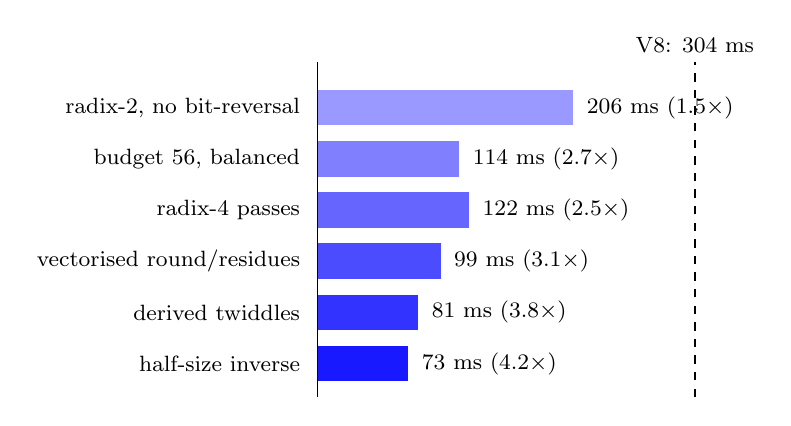
\begin{tikzpicture}[font=\footnotesize]
\fill[blue!40] (0,0.000) rectangle (3.246,0.450);
\node[anchor=east] at (-0.100,0.225) {radix-2, no bit-reversal};
\node[anchor=west] at (3.296,0.225) {206 ms (1.5$\times$)};
\fill[blue!50] (0,-0.650) rectangle (1.796,-0.200);
\node[anchor=east] at (-0.100,-0.425) {budget 56, balanced};
\node[anchor=west] at (1.846,-0.425) {114 ms (2.7$\times$)};
\fill[blue!60] (0,-1.300) rectangle (1.922,-0.850);
\node[anchor=east] at (-0.100,-1.075) {radix-4 passes};
\node[anchor=west] at (1.972,-1.075) {122 ms (2.5$\times$)};
\fill[blue!70] (0,-1.950) rectangle (1.560,-1.500);
\node[anchor=east] at (-0.100,-1.725) {vectorised round/residues};
\node[anchor=west] at (1.610,-1.725) {99 ms (3.1$\times$)};
\fill[blue!80] (0,-2.600) rectangle (1.276,-2.150);
\node[anchor=east] at (-0.100,-2.375) {derived twiddles};
\node[anchor=west] at (1.326,-2.375) {81 ms (3.8$\times$)};
\fill[blue!90] (0,-3.250) rectangle (1.150,-2.800);
\node[anchor=east] at (-0.100,-3.025) {half-size inverse};
\node[anchor=west] at (1.200,-3.025) {73 ms (4.2$\times$)};
\draw[black,thick,dashed] (4.790,-3.450) -- (4.790,0.8) node[above] {V8: 304 ms};
\draw (0,-3.450) -- (0,0.8);
\end{tikzpicture}}
